In the world of marine and underwater robotics we can indentify two categories of elements: mobile marine objects (MMO) and flexible tethers (FT). Mobile marine objects include surface vessels, submarines and remotely operated vehicles. Flexible tethers can represent umbilical cables, traction cables and anchor chains in the marine environment. They constitute all the necessary elements to achieve a mission in this environment which is sometimes quite difficult to explore.

The simulation of moving marine objects is something well known. We are now able to know from state equations the behavior of robots in their environment, and these equations are known for ships, submarines, sailboats, etc...

On the other hand, determining the behavior of a flexible tether becomes more complicated. Indeed, the equation of motion of these objects involves non-linear partial differential equations and the motion between the different objects in the environment are dynamically dependent. It is well illustrated that if the boat moves, it will induce a motion in the flexible tether that will modify the trajectory of the remotely operated vehicle. This is why it is difficult to find a way to model flexible tethers in underwater environments.

\begin{figure}
	\centering
	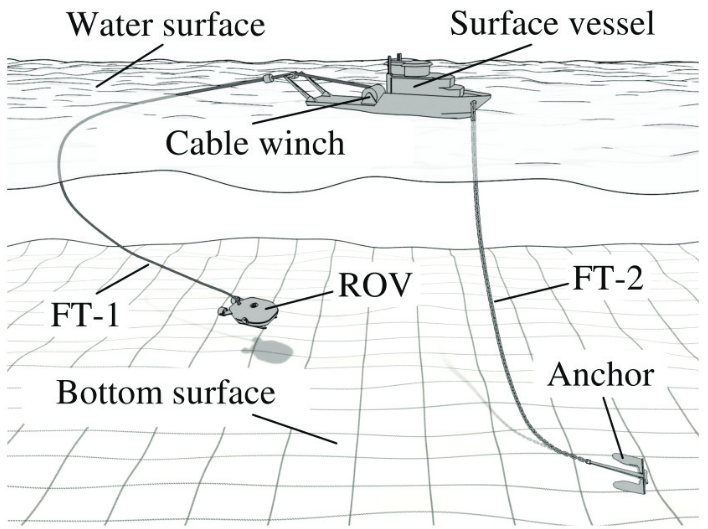
\includegraphics[width=0.4\textwidth]{imgs/underwater_environment.png}
	\caption{Example of a complex underwater environment }
	\label{fig:underwater_environment}
\end{figure}